% This text is proprietary.
% It's a part of presentation made by myself.
% It may not used commercial.
% The noncommercial use such as private and study is free
% Dec 2007
% Author: Sascha Frank 
% University Freiburg 
% www.informatik.uni-freiburg.de/~frank/
%
% 
\documentclass{beamer}
\setbeamertemplate{navigation symbols}{}


\usetheme{Warsaw}
\usepackage{listings}
\beamersetuncovermixins{\opaqueness<1>{25}}{\opaqueness<2->{15}}
\begin{document}
\title{Benchmark Studies of Various Deep Learning Architecture}  
\author{Irfan Nur Afif}
\date{\today} 


\begin{frame}
\titlepage
\end{frame}

\begin{frame}\frametitle{Table of contents}\tableofcontents
\end{frame} 


\section{Introduction} 
%\begin{frame}\frametitle{Title} 
%Each frame should have a title.
%\end{frame}
\subsection{Context \& Motivation }
\begin{frame}\frametitle{Context \& Motivation}
\begin{itemize}
	\item Deep Learning has proven to be doing well in solving complex classification task such as image and speech recognition.
	\item In this research, we are interested to investigate deep learning for image data (CNN).
	\item Main problem: no exact guidelines on designing a deep learning architecture. 
	\item Another problem: we rarely see the performance comparison of various deep learning architecture for the same standard datasets
\end{itemize}
\end{frame}
\begin{frame}\frametitle{Context \& Motivation}
   
To solve this problem, we propose a benchmarking studies of multiple deep learning architecture on many image datasets. The goal of the research is to have a benchmark analysis of various deep learning architecture performance on multiple image datasets.
\end{frame}
\subsection{Research Question}
\begin{frame}\frametitle{Research Question}    
\begin{itemize}
\item The works tries to answer the following research question: 

"How does the performance comparison of deep learning architecture model looks like for a given image classification dataset?" 

\item There are also some sub-questions to solve the main research questions, which are:
\begin{enumerate}
\item Which architecture that works bests for a given datasets?
\item What kind of datasets characteristics that makes a deep learning architecture works well?
\item Is there any architecture that generally works well for image classification?
\end{enumerate}
\end{itemize}
\end{frame}


\section{Literature Study} 
\subsection{Deep Learning}
\begin{frame}\frametitle{Convolutional Neural Network}
\begin{itemize}
\item Deep learning technique for image data. 
\item Three lypes of layers: convolitional layer, subsampling layer (maxpooling, average pooling) and fully connected layers.
\item Sometimes there is a dropout layer.
\end{itemize} 
\end{frame}
\begin{frame}\frametitle{LeNet-5}
\begin{itemize}
	\item Proposed by Yann LeCun, et al. (1998)
	\item Key idea: 7 layers, combination of 5x5 filter size in convolutional layer and 2x2 subsampling layer. 
\end{itemize}
\begin{figure}[h]
	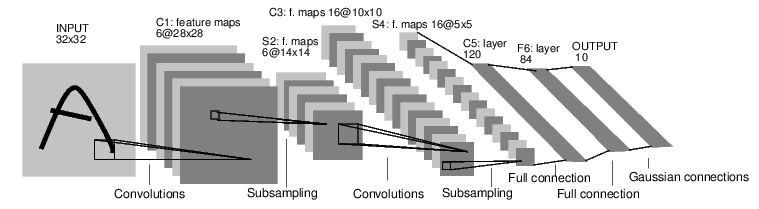
\includegraphics[scale=0.4]{figures/lenet5}
	\centering
	%\caption{LeNet-5 Architecture \cite{lecun1998gradient}}
	\label{fig:lenet5}
\end{figure}

\end{frame}
\begin{frame}\frametitle{Alex-Net}
\begin{itemize}
	\item Proposed by Alex Krizhevsky, et al. (2012)
	\item Winner of ILSVRC 2012
	\item Tested on ILSVRC 2012 dataset, achieves top 5 test error rate of 15.4\%
\end{itemize}
\begin{figure}[h]
	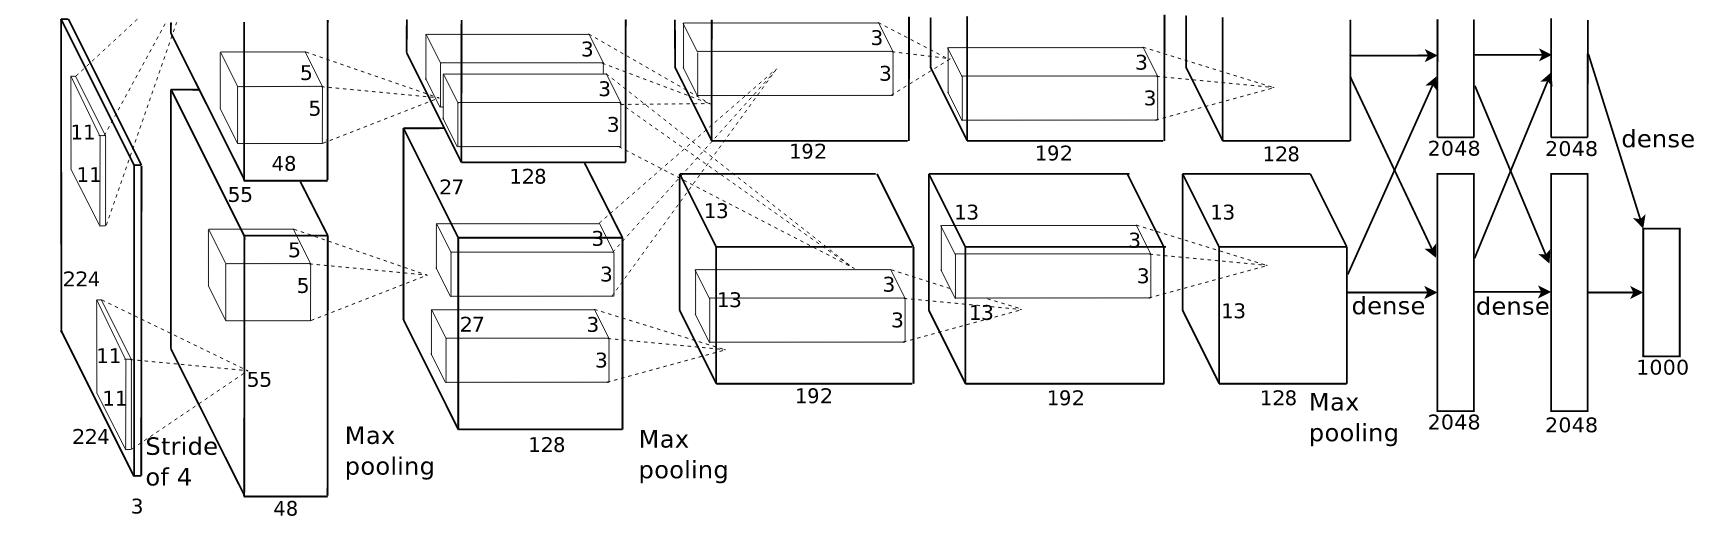
\includegraphics[scale=0.15]{figures/alexnet}
	\centering
	\label{fig:alexnet}
\end{figure}
\end{frame}

%\begin{frame}\frametitle{ZF-Net}
%\begin{itemize}
%	\item Proposed by Zeiler and Fergus
%	\item Winner of ILSVRC 2013
%	\item Tested on ILSVRC 2012 dataset, achieves top 5 test error rate of 11.2\%
%\end{itemize}
%\begin{figure}[h]
%	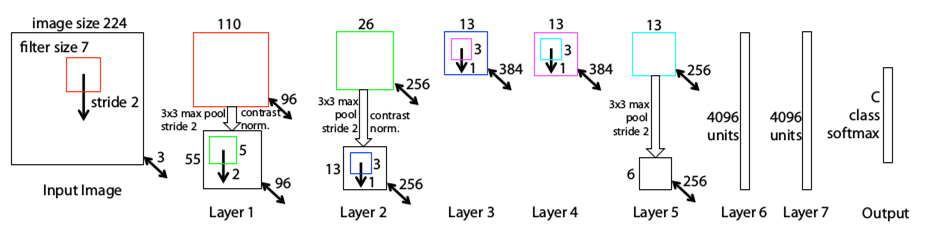
\includegraphics[scale=0.4]{figures/zfnet}
%	\centering
	%\caption{ZF Net Architecture \cite{zeiler2014visualizing}}
%	\label{fig:zf}
%\end{figure}
%\end{frame}
\begin{frame}\frametitle{VGG-Net}
\begin{itemize}
	\item Proposed by Karen Simonyan and Andrew Zisserman.
	\item Key idea: 3x3 filters (stride and pad of 1), 2x2 maxpooling layers (stride of 2), 11-19 layers.
	\item Tested on ILSVRC 2012 dataset, achieves top 5 test error rate of 6.8\%
\end{itemize}
\begin{figure}[h]
	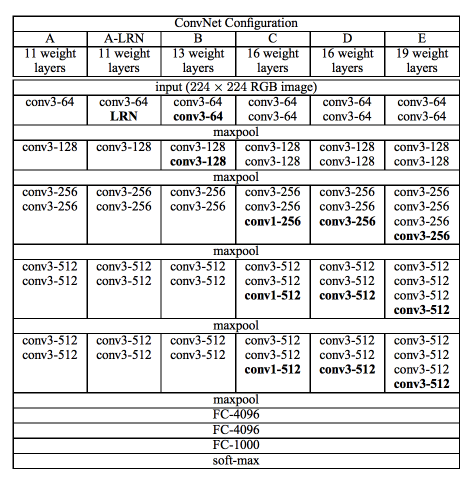
\includegraphics[scale=0.25]{figures/vggnet}
	\centering
	%\caption{VGG Net Configuration \cite{simonyan2014very}}
	\label{fig:vgg}
\end{figure}
\end{frame}
\begin{frame}\frametitle{Res-Net}
\begin{itemize}
	\item Proposed by Microsoft, winner of ILSVRC 2015.
	\item Key idea: very deep network: up to 1202 layers using 3x3 filter size in convolutional layer.
	\item Achieved 6.43\% error rate on CIFAR-10 (110 layers) and 3.6\% error rate on ILSVRC 2015 dataset. 
\end{itemize}
\end{frame}
\subsection{Datasets}
\begin{frame}\frametitle{MNIST}
\begin{itemize}
	\item Handwritten digits datasets
	with 784 features (28x28 grayscale images)
	\item 10 classes, 60,000 training examples and
	10,000 testing examples.
\end{itemize}
\begin{figure}[h]
	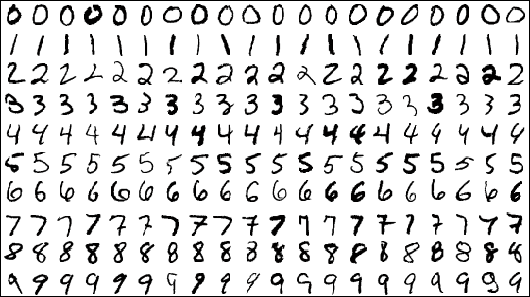
\includegraphics[scale=0.3]{figures/mnist}
	\centering
	%\caption{An example of MNIST dataset}
	\label{fig:mnist}
\end{figure}
\end{frame}

\begin{frame}\frametitle{Fashion MNIST}
\begin{itemize}
\item Zalando's article images datasets
with 784 features (28x28 grayscale images)
\item Very similar to MNIST
\item 10 classes, 60,000 training examples and
10,000 testing examples.
\end{itemize}
\begin{figure}[h]
	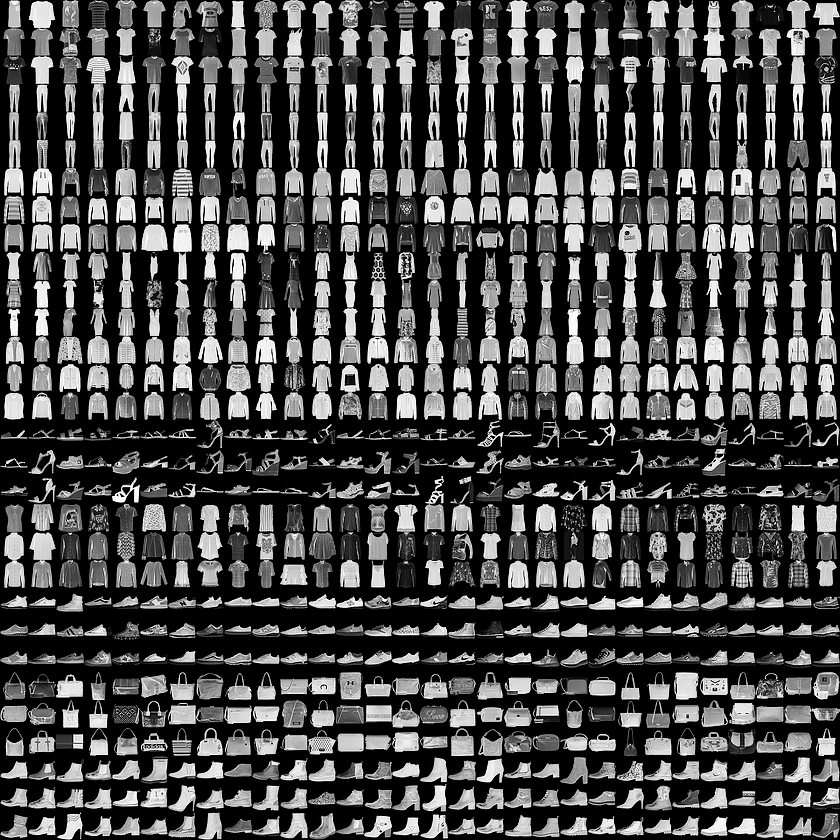
\includegraphics[scale=0.25]{figures/fashion-mnist}
	\centering
	%\caption{Fashion-MNIST sprite. Each three rows in the sprite corresponds to a single class example. \cite{xiao2017/online}}
	\label{fig:fashionmnist}
\end{figure}
\end{frame}
\begin{frame}\frametitle{CIFAR-10}
\begin{itemize}
	\item Labeled subset of the 80 million tiny images dataset, collected by Alex
	Krizhevsky, Vinod Nair, and Geoffrey Hinton 
	\item 10 classes: airplane, automobile, bird, cat, deer, dog, frog, horse, ship, truck.
	\item Colored images with a size of 32x32 pixels.
	\item 50,000 training examples and
	10,000 testing examples.
\end{itemize}
\begin{figure}[h]
	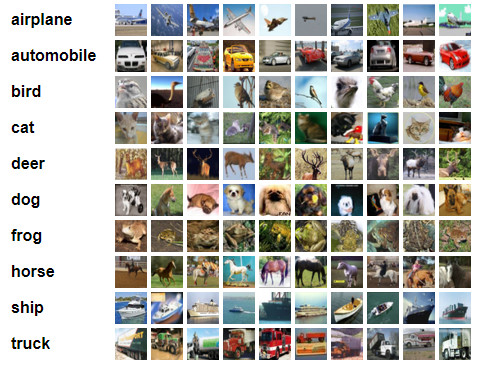
\includegraphics[scale=0.3]{figures/cifar10}
	\centering
	%\caption{Example of CIFAR-10 dataset \cite{krizhevsky2009learning}}
	\label{fig:cifar10}
\end{figure}

\end{frame}


\begin{frame}\frametitle{SVHN}
\begin{itemize}
	\item The Street View House Numbers (SVHN) Dataset is a dataset obtained from house numbers in Google Street View images
	\item Colored images with a size of 32x32 pixels.
	\item 10 classes, 73257 digits for training, 26032 digits for testing.
\end{itemize}
\begin{figure}[h]
	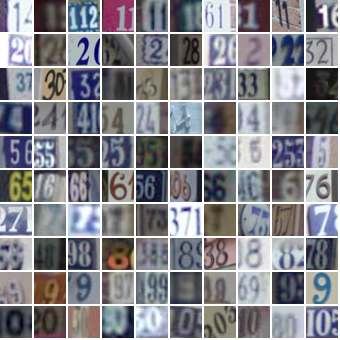
\includegraphics[scale=0.4]{figures/svhn}
	\centering
	%\caption{Examples of SVHN datasets \cite{netzer2011reading}}
	\label{fig:svhn}
\end{figure}
\end{frame}

\section{Experiment} 
\subsection{Architecture Implementation}
\begin{frame}\frametitle{LeNet}
\begin{figure}[h]
	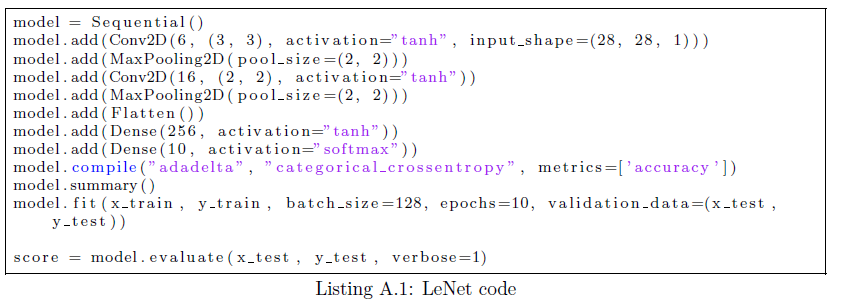
\includegraphics[scale=0.5]{figures/lenet_code}
	\centering
	\label{fig:lenet_arch}
\end{figure}

\end{frame}
\begin{frame}\frametitle{VGG-Net}
We adopt simplified VGG-Net with 4 convolutional layers 
\begin{figure}[h]
	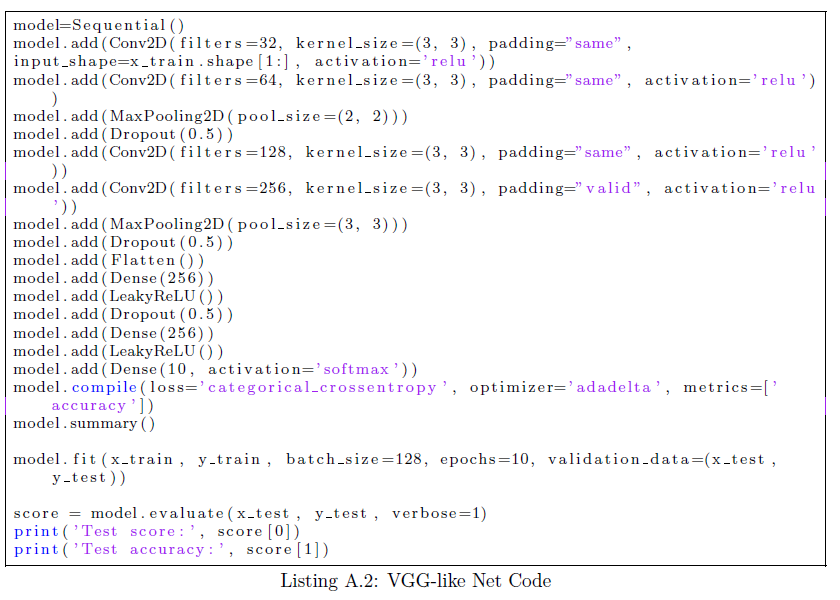
\includegraphics[scale=0.4]{figures/vggnet_code}
	\centering
	\label{fig:vggnet_arch}
\end{figure}
\end{frame}
\begin{frame}\frametitle{ResNetV1}
\begin{itemize}
	\item We implement the simplest form of ResNetV1 which is ResNet20V1 due to hardware constraint.   
	\item In this variation, there are 20 stacks of "resnet block". Each block consists of 2 x (3 x 3) Convolution-Batch Normalization-ReLU layer.
	\item In applying ResNet, we use ResNet builder library that are available at \href{https://github.com/keras-team/keras/blob/master/examples/cifar10\_resnet.py}{https://github.com/keras-team/keras/blob/master/examples/cifar10\_resnet.py}.
\end{itemize} 
\end{frame}
\begin{frame}\frametitle{ResNetV2}
\begin{itemize}
	\item  The difference of ResNet V2 and V1 is that, in V2 each block consists of  (1 x 1)-(3 x 3)-(1 x 1) Batch Normalization-ReLU-Convolution layer. 
	\item At the beginning of each 'stage', the feature map size is halved (downsampled) by a convolutional layer with strides=2, while the number of filter maps is doubled. Within each 'stage', the layers have the same number filters and the
	same filter map sizes. 
\end{itemize} 
\end{frame}
\begin{frame}\frametitle{Alex-Net/SqueezeNet}
\begin{itemize}
	\item Initially we plan to implement AlexNet, but when we try to implement it on the current machine we failed to implement it because the number of trainable parameters are too big. 
	\item Then, we discover SqueezeNet, a simpler version of AlexNet that could achieve similar accuracy with less memory resource and training time. 
\end{itemize} 
\end{frame}
\begin{frame}\frametitle{Alex-Net/SqueezeNet}
\begin{itemize}
	\item The architecture consists of convoultional layer and fire module.  
	\item  A fire module consists of 1x1 convolutional layer followed by a mix of 1x1 and 3x3 convolution layer.
	\item Then, it gradually increase the number of filters per fire module from the beginning to the end of the network.
	\item SqueezeNet performs max-pooling with a stride of 2 after layers conv1, fire4, fire8, and conv10.
\end{itemize} 
\end{frame}
\begin{frame}\frametitle{Alex-Net/SqueezeNet}
\begin{figure}[h]
	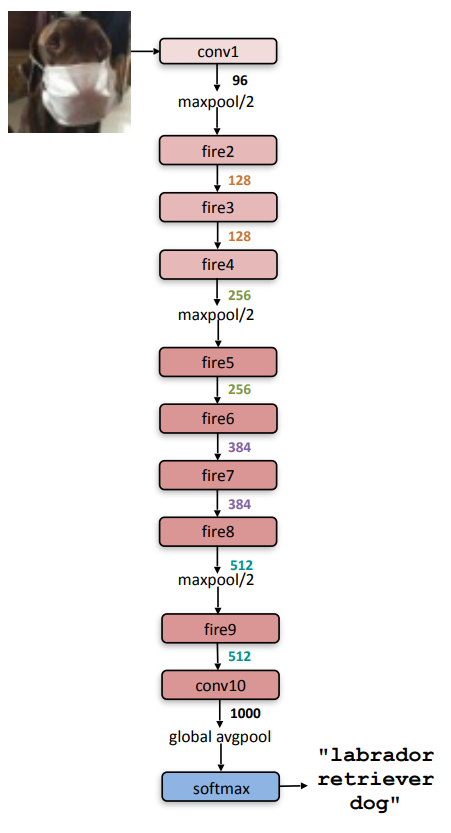
\includegraphics[scale=0.3]{figures/squeezenet}
	\centering
	\caption{SqueezeNet architecture}
	\label{fig:squeezenet_arch}
\end{figure}
\end{frame}
\subsection{Data Preprocessing}
\begin{frame}[fragile]\frametitle{MNIST, Fashion-MNIST, CIFAR-10}
\begin{figure}[h]
	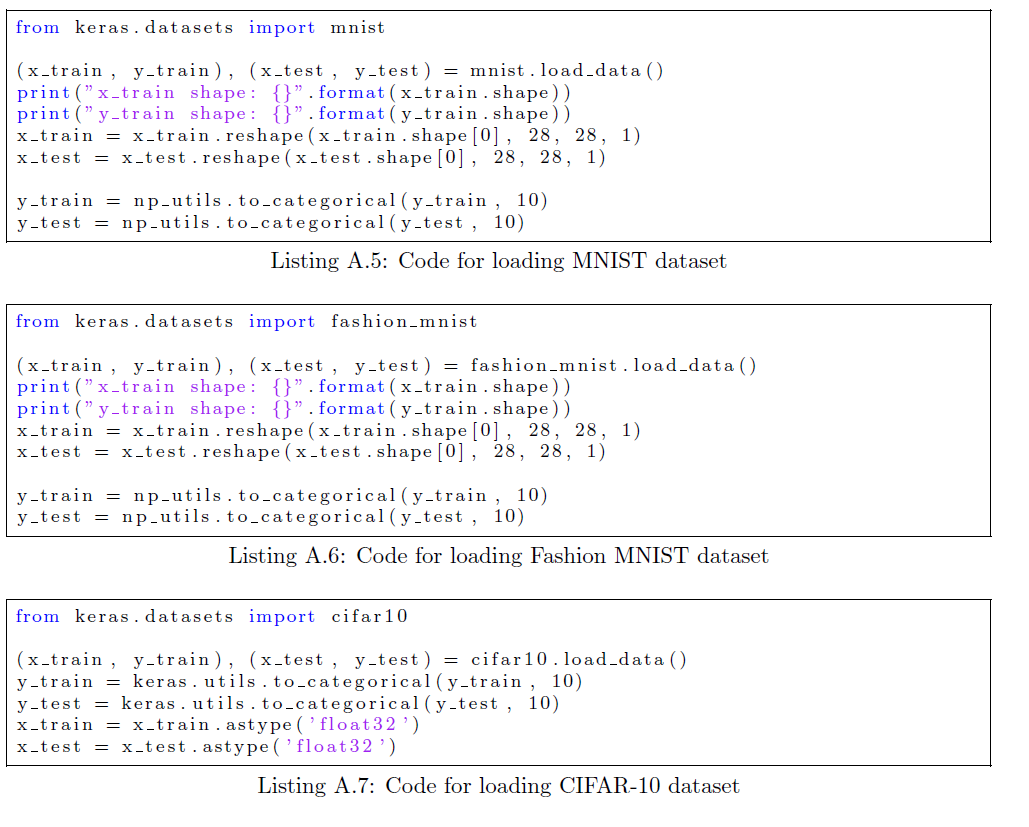
\includegraphics[scale=0.3]{figures/loaddata}
	\centering
	\label{fig:loaddata}
\end{figure}
\end{frame}
\begin{frame}\frametitle{SVHN}
\begin{figure}[h]
	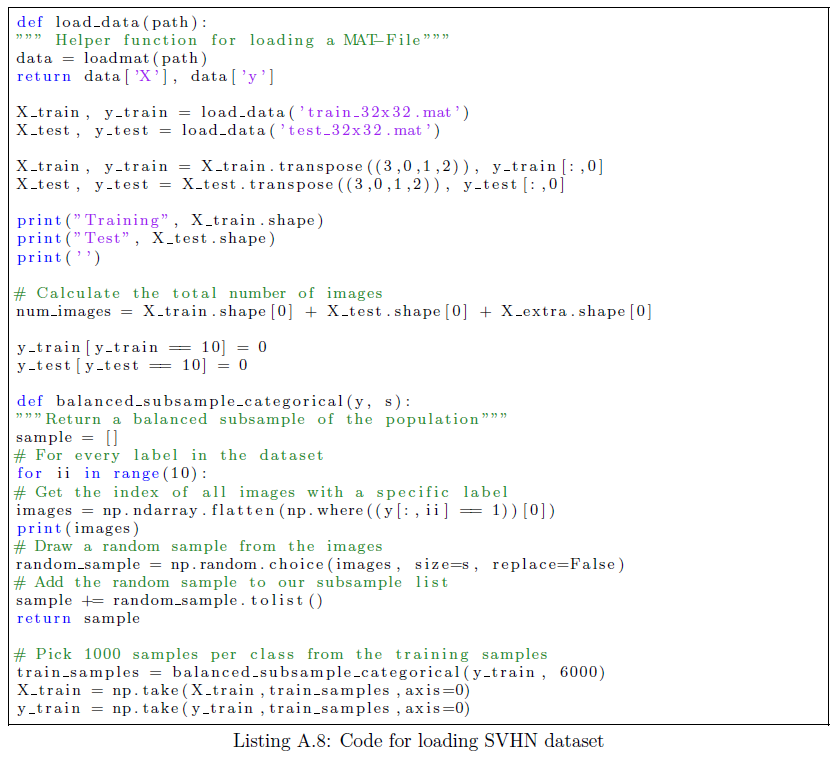
\includegraphics[scale=0.3]{figures/loadsvhn}
	\centering
	\label{fig:loadsvhn}
\end{figure}
\end{frame}

\section{Result and Discussion} 
\subsection{Result}
\begin{frame}\frametitle{Accuracy}
\begin{table}	
	\centering
	\begin{tabular}{ |c|c|c|c|c| } 
		\hline
		& MNIST & Fashion MNIST & CIFAR-10 & SVHN \\ 
		\hline
		LeNet-5	& 0.9834 & 0.8816 & 0.6561 & 0.809\\
		\hline 
		VGG-like & 0.9946 & 0.91 & 0.4075 & 0.067\\ 
		\hline
		Resnet20v1 & 0.9246 & 0.592 & 0.7567 & 0.866\\ 
		\hline
		Resnet20v2 & 0.9222 & 0.8425 & 0.679 & 0.893\\
		\hline
		SqueezeNet & 0.9858 & 0.8813 & 0.555 & 0.775\\
		\hline
	\end{tabular}
	\caption{Accuracy table}
	\label{tab:accuracy}
\end{table}
\end{frame}
\begin{frame}\frametitle{Memory Resource}
\begin{figure}[h]
	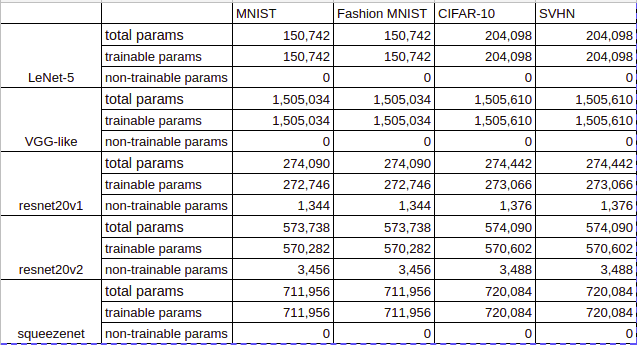
\includegraphics[scale=0.4]{figures/params}
	\centering
	\label{fig:params}
\end{figure}
\end{frame}
\begin{frame}\frametitle{Time Consumption}
\begin{table}
	\centering
	\begin{tabular}{ |c|c|c|c|c| } 
		\hline
		& MNIST & Fashion MNIST & CIFAR-10 & SVHN \\ 
		\hline
		LeNet-5	& 220s & 220s & 330s & 220s\\
		\hline 
		VGG-like & 4986s	& 4469s & 6816s & 6526s\\ 
		\hline
		Resnet20v1 & 7970s & 7909s	& 7204s & 9310s\\ 
		\hline
		Resnet20v2 & 13900s & 	13910s & 	12060s & 	15693s\\
		\hline
		SqueezeNet & 13800s & 	13907s & 	13630s & 	17550s\\
		\hline
	\end{tabular}
	%\caption{Execution time for each experiment.}
	\caption{Execution time table}
	\label{tab:times}
\end{table}
\end{frame}

\subsection{Discussion}
\begin{frame}
Main Question: "How does the performance comparison of deep learning architecture
model looks like for a given image classification dataset?"
\begin{itemize}
	\item From the execution time, it is shown that LeNet is the fastest network to train (around 22 seconds/epoch) followed by Simplified VGG-Net and Resnet20V1. 
	\item ResNet20V2 and SqueezeNet are the most time consuming network to train. 
	\item LeNet is also the least memory consuming network, followed by ResNet20V1, ResNet20V2, SqueezeNet and Simplified VGG network respectively. 
	\item In terms of accuracy, there are no single architecture that produces the best result for each datasets. 
\end{itemize} 
\end{frame}
\begin{frame}
SQ 1: Which architecture that works bests for a given datasets?
\begin{itemize}
	\item We can see that Simplified VGG architecture performs best on MNIST and Fashion MNIST dataset. 
	\item ResNet20V1 and ResNet20V2 performs best on CIFAR-10 and SVHN dataset respectively. 
	\item In terms of memory usage and time consumption, it is shown that LeNet produces the simplest network for all datasets.
\end{itemize}
\end{frame}
\begin{frame}
SQ 2: What kind of datasets characteristics that makes a deep learning architecture works well?
\begin{itemize}
	\item LeNet generally works well across all dataset except CIFAR-10. With a low amount of training time and low memory consumption, this network can be an initial tester for classifying an image dataset.
	\item Simplified VGGNet performs well on grayscale dataset: MNIST and Fashion-MNIST but gives low accuracy for colored dataset: CIFAR-10 and SVHN dataset. This is an indication that maybe VGG-like architecture performs better on grayscale dataset compared to colored dataset. Also since CIFAR-10 and SVHN image size are bigger than MNIST and Fashion-MNIST, it could be an indication that Simplified VGG-Net works better on smaller image dataset.
\end{itemize}
\end{frame}
\begin{frame}
SQ 2: What kind of datasets characteristics that makes a deep learning architecture works well?
\begin{itemize}
	\item ResNet20v1 gives high accuracy in digit recognition dataset: MNIST and SVHN but performs worse on object recognition dataset: Fashion-MNIST and CIFAR-10. It could be that the architecture is suitable for digit recognition dataset compared to object-recognition dataset.
	\item 	ResNet20v2 which is a refinement from ResNet20v1 does not always increase the performance of ResNet20v1. However, on Fashion MNIST dataset, the improvemance is quite huge, around 25\% accuracy. This architecture gives the most stable performance compared to other architecture, with the lowest accuracy is 67.9\% on CIFAR-10 dataset. 
\end{itemize}
\end{frame}
\begin{frame}
SQ 2: What kind of datasets characteristics that makes a deep learning architecture works well?
\begin{itemize}
	\item SqueezeNet is the most time consuming network to train, however it does not yields the best solution for any dataset. We need to test it on bigger epoch and see whether it can produces better result or not. If it is indeed yields a better result, then we could say that this architecture has slow improvement rate for every epoch. If is not, then we could say that this architecture is not suitable for these datasets. 
\end{itemize}
\end{frame}
\begin{frame}
SQ 3: Is there any architecture that generally works well for image classification?
	
	There are not a single architecture that gives best performance across all datasets. However, based on table \ref{tab:accuracy} we can see that in general, ResNet20v2 gives the most stable and good performance on average across all datasets. This does not means that this architecture always gives stable and good performance on most datasets. Further experiment needs to be done to confirm this findings.
\end{frame}

	


\begin{frame}\frametitle{Limitation}
\begin{itemize}
	\item Due to the time and hardware contraint, this studies was conducted only on 4 datasets and 5 architectures.
	\item  A more powerful machine/hardware is needed to do further benchmarking studies. As an example, applying ResNet20V1 on CIFAR-10 dataset, using current machine took 720 seconds/epoch while applying it on GTX1080Ti took 35 seconds/epoch (according to \href{https://github.com/keras-team/keras/blob/master/examples/cifar10\_resnet.py}{https://github.com/keras-team/keras/blob/master/examples/cifar10\_resnet.py}).
	\item  Faster experiment means better classification performance and more architecture and dataset that could be implemented. 
\end{itemize}
\end{frame}

\section{Conclusion}
\subsection{Conclusion}
\begin{frame}\frametitle{Conclusion}
\begin{enumerate}
	\item There are no single architecture that gives the best performance across all tested dataset.
	\item LeNet is the most simple yet powerful network.
	This networks can become the tester network for in an image dataset because of its low time to train and memory to use. We can use LeNet classification result as initial performance benchmarks compared to other sophisticated architecture.
	\item Simplified VGGNet performs well on grayscale dataset compared to colored-dataset. Also it performs better on smaller image. It can achieve an accuracy of 99.46\% and 91\% on MNIST and Fashion-MNIST dataset respectively.
	
\end{enumerate}
\end{frame}

\begin{frame}\frametitle{Conclusion}
\begin{enumerate}
	\setcounter{enumi}{3}
	\item ResNetV1 works better in digit recognition compared to object recognition. It can achieve an accuracy of 92.46\% and 86.6\% on MNIST and SVHN dataset.
	\item ResNetV2 does not always increase the performance of ResNetv1. However, on Fashion MNIST dataset, the improvemance is quite huge, around 25\% accuracy.
	\item ResNetV2 gives quite good and stable performance compared to other network.
	\item SqueezeNet consumes the most memory and time to train but does not yields the best classification performance on any dataset.
\end{enumerate}
\end{frame}
\subsection{Future Works}
\begin{frame}\frametitle{Future Works}
\begin{itemize}
	 \item Further works can be done by doing larger benchmark studies by applying more architecture and more dataset in the experiment. 
	 \item By doing this, we can also verifying the initial findings that was presented in the conclusion. Increasing the number of epoch can be a good way to verify the initial finding that was presented here. 
	 \item Furthermore, we only see memory usage, time consumption and accuracy for the experiment. Other matrices should be explored for future works.
\end{itemize}
\end{frame}


\end{document}